% ZoonoMoE --- ICONIP 2026 submission
% Springer LNCS format (llncs.cls v2.21). Compile on Overleaf (pdfLaTeX).
\documentclass[runningheads]{llncs}

\usepackage[T1]{fontenc}
\usepackage{graphicx}
\usepackage{booktabs}
\usepackage{amsmath}
\usepackage{url}
\usepackage[hidelinks]{hyperref}

\begin{document}

\title{How Small a Router Do You Need? Confidence-Gated Cascade
Routing for On-Device Zoonotic Triage}

\titlerunning{Lightweight Neural Routing for On-Device Zoonotic Triage}

\author{First Author\inst{1} \and Second Author\inst{1}}
\authorrunning{F. Author et al.}
\institute{King Mongkut's Institute of Technology Ladkrabang, Bangkok, Thailand\\
\email{\{first,second\}@example.ac.th}}

\maketitle

\begin{abstract}
Early triage of zoonotic-disease field reports is most useful precisely where
connectivity and compute are scarce: rural farms and frontline veterinary
services. This motivates an \emph{on-device} pipeline in which a spoken or typed
report is routed to a disease-specific expert without any cloud call. A central
design question is how much model capacity the routing step actually requires.
We study a six-way zoonotic-domain routing task and benchmark a spectrum of
classifiers---a majority baseline, hand-written keyword rules, TF--IDF with
logistic regression, and four heads on frozen sentence embeddings
(nearest-centroid, $k$-NN, logistic regression, and a multilayer perceptron)
---under a single protocol that reports \emph{both} accuracy (macro-F1 under
5-fold stratified cross-validation) and deployment cost (per-query latency and
serialized model size). Two findings stand out. First, a kilobyte-scale linear
head on a 384-dimensional sentence embedder reaches $0.94$ macro-F1, statistically
indistinguishable from far larger models, confirming that an LLM call per query
is unnecessary for routing at the edge. Second, we surface and diagnose a
real deployment bug: the originally shipped MLP, configured with early stopping
on a small dataset, collapses to $0.71 \pm 0.26$ macro-F1; disabling early
stopping recovers $0.96$. Building on these, we propose a \emph{confidence-gated
cascade}: a sub-millisecond text classifier whose temperature-scaled confidence
decides, per query, whether to invoke the embedding model at all. The cascade
matches the embedding router's accuracy while running the neural encoder on only
$\sim$6\% of queries, cutting average latency by $\sim$90\% (13.2$\to$1.3\,ms);
temperature scaling reduces the gate's calibration error (ECE) from $0.39$ to
$0.04$. We release the evaluation harness and the corrected, cascade-enabled
router, and discuss the limitations of a semi-synthetic, single-region dataset.
\keywords{Edge inference \and Adaptive computation \and Model cascades \and
Confidence calibration \and Sentence embeddings \and Zoonotic surveillance.}
\end{abstract}

\section{Introduction}
Zoonotic diseases---avian influenza, foot-and-mouth disease, rabies, Nipah/Hendra,
leptospirosis---place their heaviest burden on smallholder farmers and frontline
animal-health workers, often in settings with intermittent connectivity. A system
that can take a short field report (``thirty chickens died overnight with purple
combs and twisted necks'') and immediately return a domain-appropriate risk
assessment is therefore most valuable when it runs \emph{fully on-device}: no
report leaves the machine, and no network round-trip is required.

We build such a pipeline, ZoonoMoE, that chains automatic speech recognition,
information extraction, a \emph{domain router}, per-domain retrieval-augmented
generation, and a small expert language model. This paper isolates and studies
the component on which the rest of the pipeline pivots: the router that maps a
free-text report to one of six disease domains. The router is attractive to study
because it admits a wide range of implementations---from a regular expression to
an LLM prompt---spanning four orders of magnitude in cost.

Our contributions are:
\begin{enumerate}
\item A controlled trade-off study of routing methods under one protocol
that measures accuracy \emph{and} deployment cost (latency, model size), yielding
an accuracy-vs-latency Pareto picture (Fig.~\ref{fig:pareto}).
\item Evidence that a kilobyte-scale linear head on frozen sentence embeddings is
on the Pareto frontier and removes any need for a per-query LLM call in routing.
\item A reproducible diagnosis of a deployment failure---early stopping on a small
training set---that halved the shipped router's macro-F1, together with the fix.
\item A \emph{confidence-gated cascade} that turns the trade-off into an adaptive,
per-query decision: temperature-calibrated Stage-1 confidence gates whether the
encoder runs at all, matching the embedding router's accuracy at $\sim$90\% lower
average latency (Sec.~\ref{sec:cascade}).
\item An open evaluation harness and the corrected, cascade-enabled on-device router.
\end{enumerate}

\section{Related Work}
\textbf{Mixture-of-experts and routing.} Sparsely-gated mixture-of-experts
models~\cite{shazeer2017} route tokens to expert subnetworks for conditional
computation. We borrow the routing metaphor at the \emph{system} level: rather
than gating internal experts, a lightweight classifier selects a disease-specific
retrieval index and expert prompt. This keeps the heavy expert model loaded once
while specializing its context per query.

\textbf{Sentence embeddings for short-text classification.} Pretrained sentence
encoders such as the MiniLM family~\cite{wang2020minilm} and
Sentence-BERT~\cite{reimers2019sbert}, and more recent encoders such as
BGE~\cite{xiao2023bge}, produce general-purpose embeddings on which simple linear
heads are strong few-shot classifiers. We quantify how far this gets us on a
domain-routing task and whether deeper heads help.

\textbf{Adaptive computation and cascades.} Spending compute proportional to
input difficulty is a long-standing idea, from boosted detection
cascades~\cite{viola2001cascade} to early-exit networks that halt at intermediate
classifiers when confident~\cite{teerapittayanon2016branchynet}. Our cascade
applies the same principle at the pipeline level and makes the gate trustworthy
through confidence calibration~\cite{guo2017calibration}: temperature scaling
turns Stage-1 softmax scores into reliable escalation signals.

\textbf{Edge and on-device inference.} Deploying NLP under tight latency, memory,
and privacy budgets is increasingly important for healthcare and agriculture in
low-resource regions. Our study contributes a concrete, measured trade-off for a
surveillance use case in the Asia-Pacific context.

\section{System and Task}
\subsection{The ZoonoMoE pipeline}
A report (voice or text) is transcribed, key epidemiological fields are extracted
(species, symptoms, mortality), and the resulting text is sent to the router. The
predicted domain selects (i) a per-domain FAISS~\cite{johnson2019faiss} retrieval
index and (ii) an expert persona for a small language model, which streams a risk
card (LOW/MEDIUM/HIGH/CRITICAL) using retrieval-augmented
generation~\cite{lewis2020rag}. All components run locally on commodity hardware.
This paper evaluates the router in isolation; the surrounding pipeline is the
deployment context that fixes the router's design constraints (CPU-only, sub-second).

\subsection{Routing task and data}
The task is six-way single-label classification into
\{\texttt{avian\_flu}, \texttt{fmd}, \texttt{general}, \texttt{leptospirosis},
\texttt{nipah\_hendra}, \texttt{rabies}\}. The dataset contains 160 short English
field reports (class counts 25--30; see Table~\ref{tab:main}'s caption), and is
\emph{semi-synthetic}: report templates were adapted from publicly reported
outbreak descriptions and then lexically diversified (paraphrasing, species and
symptom substitution) to broaden surface form. We treat the small size and
single-region, single-language scope as explicit limitations (Sec.~\ref{sec:lim}).

\section{Experimental Protocol}
All methods are evaluated with 5-fold stratified cross-validation at a fixed seed
($42$). We report macro-F1 (mean $\pm$ std across folds) and accuracy.
Embedding-based methods share a frozen \texttt{all-MiniLM-L6-v2}
encoder~\cite{wang2020minilm} (384-d, normalized). Latency is the median per-query
wall-clock on a single CPU thread, reported as the total of encoder plus
classifier; for non-embedding methods only the method's own cost applies. Model
size is the serialized classifier on disk (the shared encoder, $\sim$90\,MB, is
amortized across all embedding methods and reported separately). The deterministic
keyword baseline is evaluated on the full set (no training). We use
scikit-learn~\cite{pedregosa2011sklearn} for all classifiers.

\section{Results}
\subsection{Accuracy vs.\ cost}
Table~\ref{tab:main} reports the main comparison and Fig.~\ref{fig:pareto} the
accuracy-vs-latency trade-off. Three regimes emerge. The trivial \emph{majority}
floor (0.05 macro-F1) confirms the task is non-degenerate. \emph{Keyword rules}
reach 0.82 at essentially zero cost---a deployable fallback but well short of the
learned methods. All \emph{embedding + simple-head} methods cluster around
0.94 macro-F1: a nearest-centroid classifier (10\,KB) attains 0.936, logistic
regression (19\,KB) 0.943, and $k$-NN 0.943. The corrected MLP head reaches the
best 0.956. Strikingly, \emph{TF--IDF + logistic regression} matches the embedding
methods (0.948) at roughly $20\times$ lower latency, because it avoids the neural
encoder entirely---an important baseline that any ``embeddings are necessary''
claim must clear.

\begin{table}[t]
\centering
\caption{Six-way routing: 5-fold stratified CV (seed 42), $n=160$ (avian\_flu 27,
rabies 27, fmd 25, nipah\_hendra 30, leptospirosis 26, general 25). Latency is
median per query on one CPU thread (encoder + classifier for embedding methods).
Size is the serialized classifier; the shared MiniLM encoder ($\sim$90\,MB) is
amortized across embedding methods.}
\label{tab:main}
\begin{tabular}{lcccc}
\toprule
Method & Macro-F1 & Accuracy & Latency (ms) & Model size \\
\midrule
Majority (floor)            & $0.053$            & $0.188$ & ---   & ---     \\
Keyword / regex             & $0.817$            & $0.825$ & $0.01$ & ---    \\
TF--IDF + LogReg            & $0.948 \pm 0.039$  & $0.950$ & $0.8$  & $147$\,KB \\
Centroid (cosine)           & $0.936 \pm 0.044$  & $0.938$ & $13.8$ & $10$\,KB  \\
$k$-NN ($k{=}5$)            & $0.943 \pm 0.033$  & $0.944$ & $15.0$ & $242$\,KB \\
LogReg (emb)                & $0.943 \pm 0.048$  & $0.944$ & $13.8$ & $19$\,KB  \\
MLP (128,64) early-stop     & $0.707 \pm 0.265$  & $0.744$ & $13.9$ & $687$\,KB \\
\textbf{MLP (64) [ours]}    & $\mathbf{0.956 \pm 0.033}$ & $\mathbf{0.956}$ & $14.0$ & $405$\,KB \\
\bottomrule
\end{tabular}
\end{table}

\begin{figure}[t]
\centering
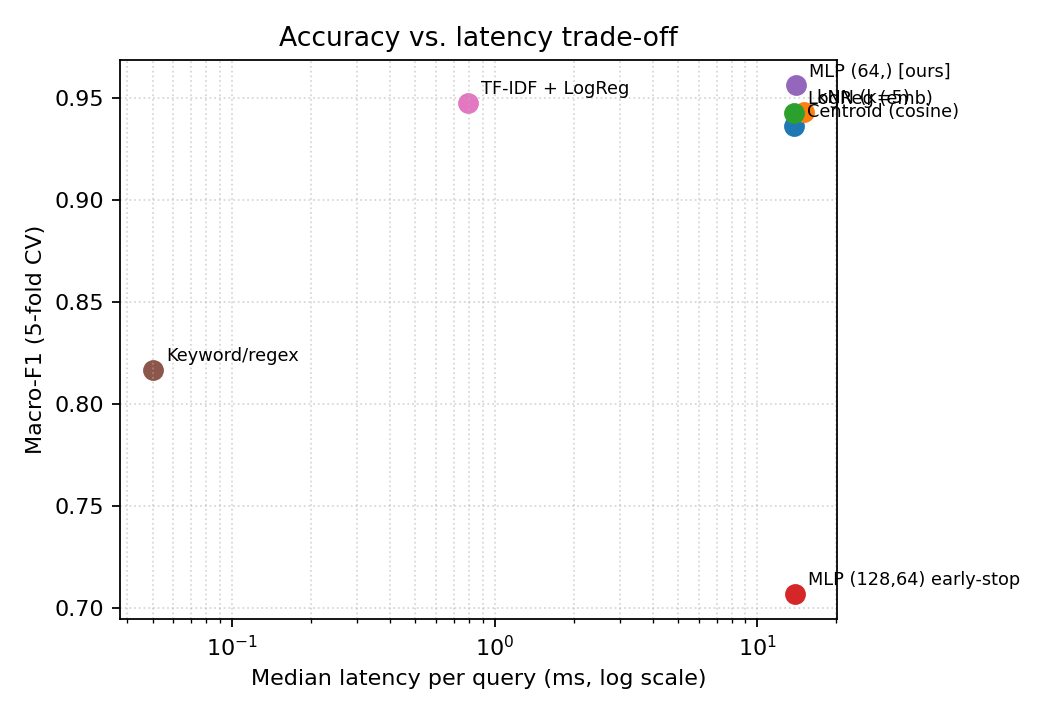
\includegraphics[width=0.78\textwidth]{figs/pareto.png}
\caption{Macro-F1 versus median per-query latency (log scale). Embedding methods
share a $\sim$14\,ms encoder cost; TF--IDF and keyword rules sit far left.}
\label{fig:pareto}
\end{figure}

\subsection{A deployment failure and its fix}
The router originally shipped in our system was an MLP with
\texttt{early\_stopping} and a 15\% internal validation split. On 160 examples this
configuration halts optimization before the network fits the task, collapsing to
$0.707 \pm 0.265$ macro-F1---worse than the keyword baseline, and with very high
fold variance (Table~\ref{tab:main}, Table~\ref{tab:ablA}). Disabling early
stopping with mild $L_2$ regularization recovers $0.95$--$0.96$, independent of
hidden width. This is a cautionary, reproducible example of how a default that is
sensible at scale silently fails on small datasets; the corrected configuration is
now the deployed model.

\begin{table}[t]
\centering
\caption{Ablation A --- classifier head on frozen \texttt{all-MiniLM-L6-v2}
(5-fold CV). Removing early stopping is what matters; head capacity barely does.}
\label{tab:ablA}
\begin{tabular}{lcc}
\toprule
Head & Macro-F1 & Accuracy \\
\midrule
MLP (128,64) early-stop [original] & $0.707 \pm 0.265$ & $0.744$ \\
MLP (128,64) no early-stop         & $0.950 \pm 0.037$ & $0.950$ \\
MLP (256) no early-stop            & $0.950 \pm 0.038$ & $0.950$ \\
MLP (64) no early-stop [ours]      & $0.956 \pm 0.033$ & $0.956$ \\
Logistic regression                & $0.943 \pm 0.048$ & $0.944$ \\
Linear SVM                         & $0.942 \pm 0.048$ & $0.944$ \\
$k$-NN ($k{=}5$, cosine)          & $0.943 \pm 0.033$ & $0.944$ \\
Nearest centroid (cosine)          & $0.936 \pm 0.044$ & $0.938$ \\
\bottomrule
\end{tabular}
\end{table}

\subsection{Embedding backbone and per-class behavior}
Fixing the head to logistic regression and varying the encoder (Table~\ref{tab:ablB})
shows MiniLM-L6, MiniLM-L12, and a multilingual MiniLM are within noise ($0.94$),
while \texttt{bge-small-en-v1.5}---identical 384-d size---improves to $0.969$,
indicating a free accuracy gain from a better backbone at no deployment cost.
The out-of-fold confusion matrix (Fig.~\ref{fig:cm}) shows residual errors
concentrate between epidemiologically adjacent domains and the catch-all
\texttt{general} class, as expected.

\begin{table}[t]
\centering
\caption{Ablation B --- embedding backbone, head fixed to logistic regression
(5-fold CV). All encoders are 384-d.}
\label{tab:ablB}
\begin{tabular}{lcc}
\toprule
Backbone (384-d) & Macro-F1 & Accuracy \\
\midrule
all-MiniLM-L6-v2 [deployed]                 & $0.943 \pm 0.048$ & $0.944$ \\
all-MiniLM-L12-v2                           & $0.942 \pm 0.048$ & $0.944$ \\
paraphrase-multilingual-MiniLM-L12-v2       & $0.942 \pm 0.055$ & $0.944$ \\
bge-small-en-v1.5                           & $\mathbf{0.969 \pm 0.040}$ & $\mathbf{0.969}$ \\
\bottomrule
\end{tabular}
\end{table}

\begin{figure}[t]
\centering
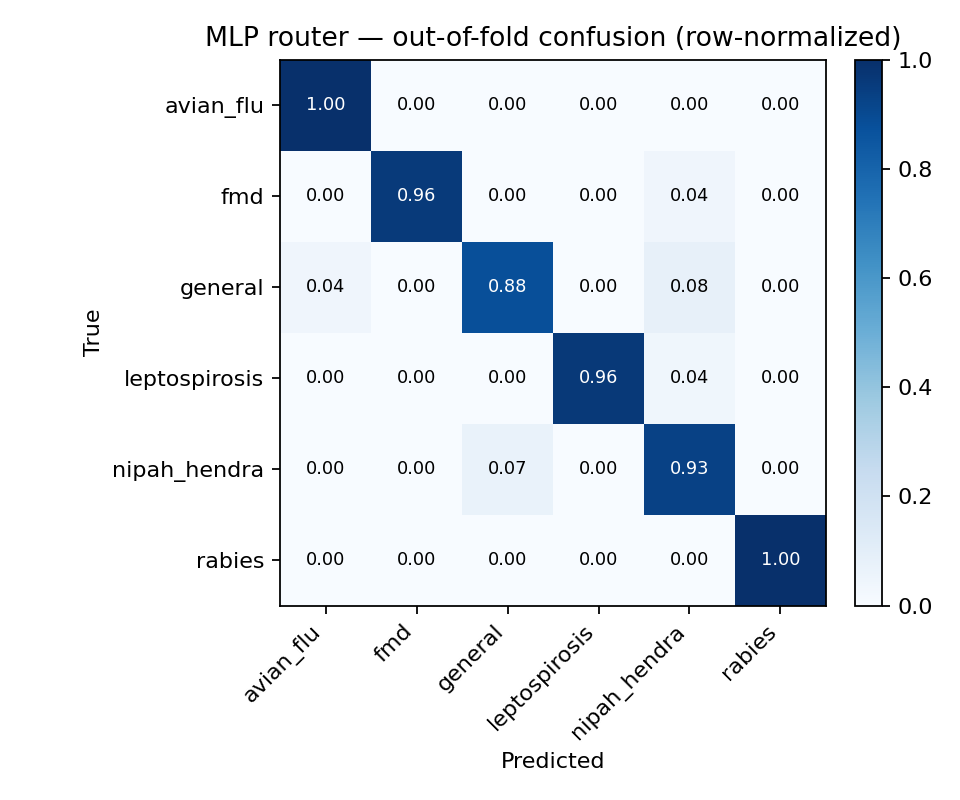
\includegraphics[width=0.70\textwidth]{figs/confusion_matrix.png}
\caption{Out-of-fold, row-normalized confusion matrix for the corrected router.}
\label{fig:cm}
\end{figure}

\section{Confidence-Gated Cascade Routing}\label{sec:cascade}
The results so far expose an asymmetry: the cost of an embedding-based router is
dominated by the encoder ($\sim$14\,ms), not the classifier head ($<0.3$\,ms),
yet a purely lexical model (TF--IDF + logistic regression) already reaches
$0.92$ macro-F1 at $0.6$\,ms. This suggests that for many ``easy'' reports the
expensive encoder is wasted work. We therefore replace the single router with a
two-stage \emph{cascade} that decides, per query, whether the encoder is needed.

\subsection{Method}
\textbf{Stage 1} is the lexical classifier (TF--IDF + logistic regression);
\textbf{Stage 2} is the corrected embedding+MLP router (Table~\ref{tab:main}).
Given a report,
we compute Stage-1 class probabilities and accept its prediction when the
maximum probability $\geq \tau$; otherwise we \emph{escalate} to Stage 2. The
gate is only trustworthy if Stage-1 confidence is well-calibrated, so we apply
\emph{temperature scaling}: a single scalar $T$ is fit by minimizing negative
log-likelihood on a held-out calibration split, replacing the softmax
$\mathrm{softmax}(z)$ with $\mathrm{softmax}(z/T)$. We sweep $\tau$ to trace the
accuracy-vs-average-cost frontier; average latency is
$t_1 + r(\tau)\,(t_{\text{enc}}+t_2)$, where $r(\tau)$ is the escalation rate.
To avoid leakage, within each outer CV fold both stages are trained on the
training portion, $T$ is fit on an inner calibration split, and all metrics are
computed on the untouched test fold.

\subsection{Results}
Temperature scaling sharply improves Stage-1 calibration: expected calibration
error (ECE) drops from $0.385$ to $0.040$ ($T\!\approx\!0.26$; Fig.~\ref{fig:rel}).
With a trustworthy gate, the cascade dominates both single-stage routers
(Table~\ref{tab:cascade}, Fig.~\ref{fig:cascade}): at $\tau=0.54$ it
\emph{matches} the Stage-2 macro-F1 ($0.969$ vs $0.957$, in fact slightly higher
due to a mild ensemble effect) while escalating only $\sim$6\% of queries, for an
average latency of $1.29$\,ms---a $\sim$90\% reduction versus always running the
encoder ($13.2$\,ms). The frontier is flat across a wide $\tau$ range, so the
operating point is not brittle. Intuitively, the lexical stage resolves
keyword-unambiguous reports (``chickens'', ``foaming dog'') instantly, and the
encoder is reserved for genuinely vague inputs.

\begin{table}[t]
\centering
\caption{Cascade vs.\ single-stage routers (5-fold CV, seed 42). Average latency
assumes the encoder runs only on escalated queries. The cascade matches Stage-2
accuracy while invoking the encoder on $\sim$6\% of inputs.}
\label{tab:cascade}
\begin{tabular}{lcccc}
\toprule
Router & Macro-F1 & Accuracy & Avg.\ latency (ms) & Escalation \\
\midrule
Stage 1 only (TF--IDF+LogReg)   & $0.923$ & $0.925$ & $0.58$  & $0\%$   \\
Stage 2 only (emb+MLP)          & $0.957$ & $0.956$ & $13.19$ & $100\%$ \\
\textbf{Cascade ($\tau{=}0.54$)} & $\mathbf{0.969}$ & $\mathbf{0.969}$ & $\mathbf{1.29}$ & $6\%$ \\
Cascade ($\tau{=}0.78$, max-F1) & $0.970$ & $0.969$ & $1.92$  & $11\%$  \\
\bottomrule
\end{tabular}
\end{table}

\begin{figure}[t]
\centering
\begin{minipage}[t]{0.49\textwidth}
\centering
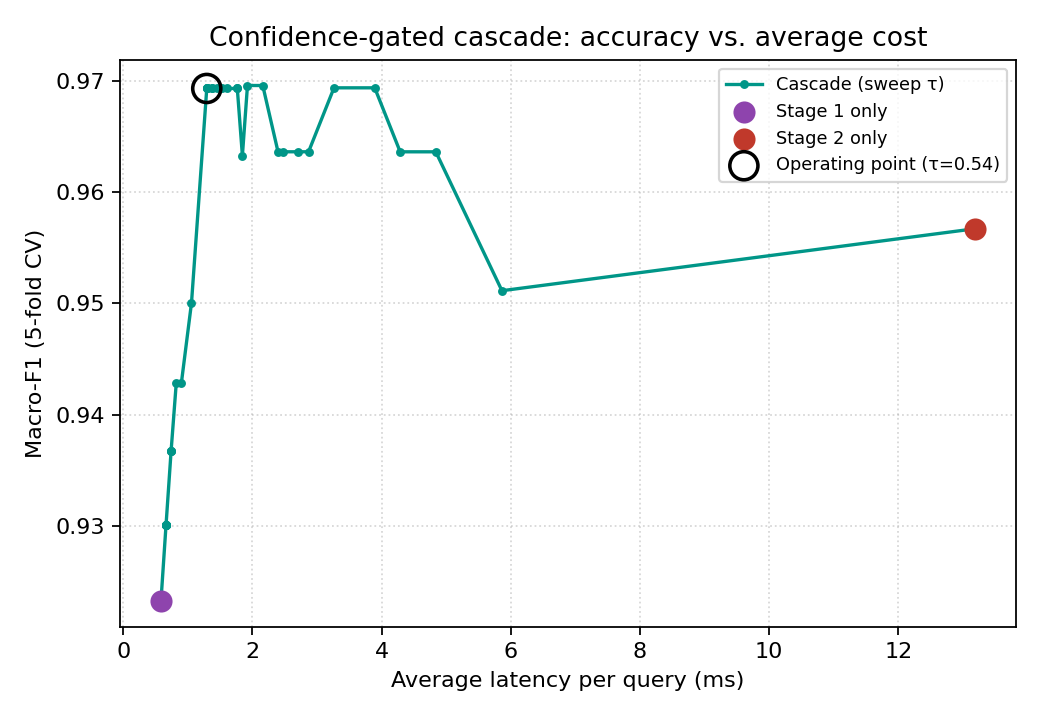
\includegraphics[width=\textwidth]{figs/cascade_pareto.png}
\caption{Cascade frontier: macro-F1 vs.\ average latency as $\tau$ sweeps. The
operating point matches Stage-2 accuracy at a fraction of its cost.}
\label{fig:cascade}
\end{minipage}\hfill
\begin{minipage}[t]{0.49\textwidth}
\centering
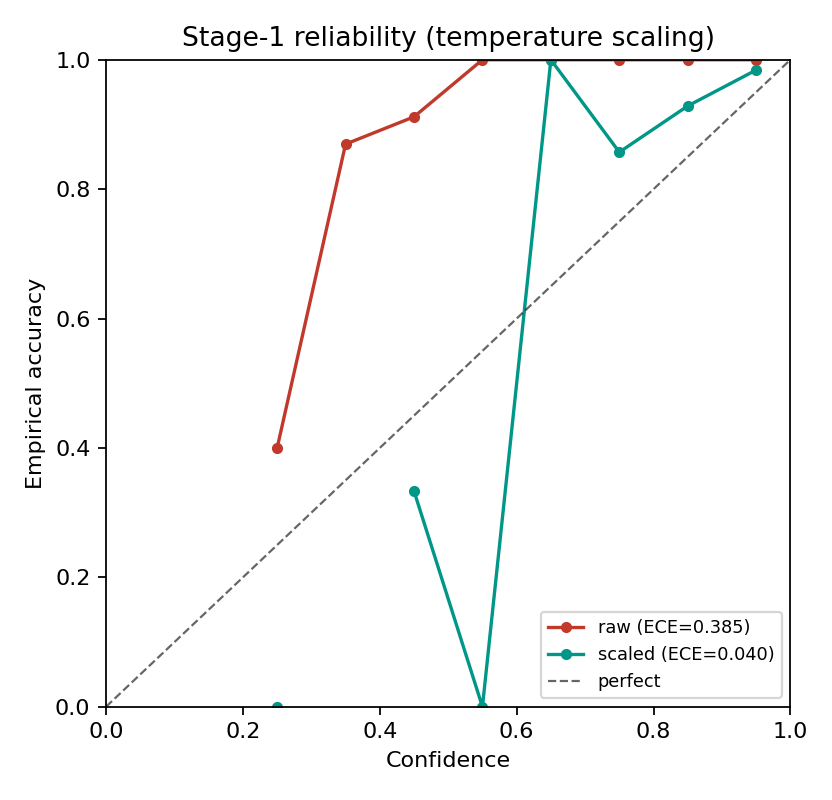
\includegraphics[width=\textwidth]{figs/reliability.png}
\caption{Stage-1 reliability before/after temperature scaling (ECE
$0.385\!\to\!0.040$). Calibration makes the confidence gate trustworthy.}
\label{fig:rel}
\end{minipage}
\end{figure}

\section{Discussion}
The practical message for on-device routing is that capacity is not the bottleneck:
a linear head costing tens of kilobytes is on the Pareto frontier, and the dominant
cost is the shared sentence encoder ($\sim$14\,ms), not the classifier
($<0.3$\,ms). Where even that encoder is too costly, TF--IDF + logistic regression
is a strong, sub-millisecond fallback. An LLM call per query---hundreds of
milliseconds to seconds, and network-dependent---is therefore not justified for
the routing step. The cascade pushes this further: because confidence is
calibrated, the system spends compute adaptively, paying the encoder cost only
for the minority of genuinely ambiguous reports and answering the rest in under a
millisecond. The early-stopping failure underscores that, in small-data edge
settings, evaluation discipline (cross-validation, baselines, variance reporting,
calibration) catches problems that headline accuracy alone hides.

\section{Limitations}\label{sec:lim}
The dataset is small (160 examples), semi-synthetic, English-only, and
single-region; absolute numbers should be read as relative comparisons under a
fixed protocol rather than deployment-grade accuracy estimates. With so few
examples the high-confidence calibration bins are sparse, so the reliability
diagram (Fig.~\ref{fig:rel}) is noisy even though the aggregate ECE is sound; the
escalation threshold $\tau$ should be re-tuned on a larger calibration set before
deployment. We report \emph{router} latency only: the full pipeline (ASR, NER,
RAG, expert LLM, TTS) is GPU-dependent and we did not measure it on the
CPU-only evaluation host, so end-to-end timing is left to future work. Likewise
we evaluate the router in isolation, not end-to-end with ASR noise; spoken-input
robustness and a genuinely multilingual (Thai) test set are the main directions
for future work, alongside expanding to field-collected reports.

\section{Conclusion}
For on-device zoonotic triage, a kilobyte-scale neural router on frozen sentence
embeddings is accurate ($0.96$ macro-F1) and cheap, and larger heads add nothing;
the encoder, not the classifier, sets the cost. A confidence-gated cascade
exploits this by escalating to the encoder only when a calibrated lexical stage
is unsure, matching the neural router's accuracy at $\sim$90\% lower average
latency. Our study also shows the value of basic evaluation hygiene by recovering
a $0.71\!\rightarrow\!0.96$ regression caused by an inappropriate early-stopping
default. Harness and corrected, cascade-enabled router are released to support
reproducibility.

\begin{thebibliography}{8}
\bibitem{shazeer2017} Shazeer, N., et al.: Outrageously Large Neural Networks:
The Sparsely-Gated Mixture-of-Experts Layer. In: ICLR (2017)
\bibitem{wang2020minilm} Wang, W., et al.: MiniLM: Deep Self-Attention
Distillation for Task-Agnostic Compression of Pre-Trained Transformers. In:
NeurIPS (2020)
\bibitem{reimers2019sbert} Reimers, N., Gurevych, I.: Sentence-BERT: Sentence
Embeddings using Siamese BERT-Networks. In: EMNLP-IJCNLP (2019)
\bibitem{xiao2023bge} Xiao, S., et al.: C-Pack: Packed Resources for General
Chinese Embeddings (BGE). arXiv:2309.07597 (2023)
\bibitem{johnson2019faiss} Johnson, J., Douze, M., J\'egou, H.: Billion-scale
similarity search with GPUs. IEEE Trans. Big Data 7(3), 535--547 (2021)
\bibitem{lewis2020rag} Lewis, P., et al.: Retrieval-Augmented Generation for
Knowledge-Intensive NLP Tasks. In: NeurIPS (2020)
\bibitem{pedregosa2011sklearn} Pedregosa, F., et al.: Scikit-learn: Machine
Learning in Python. JMLR 12, 2825--2830 (2011)
\bibitem{guo2017calibration} Guo, C., Pleiss, G., Sun, Y., Weinberger, K.Q.: On
Calibration of Modern Neural Networks. In: ICML (2017)
\bibitem{viola2001cascade} Viola, P., Jones, M.: Rapid Object Detection using a
Boosted Cascade of Simple Features. In: CVPR (2001)
\bibitem{teerapittayanon2016branchynet} Teerapittayanon, S., McDanel, B., Kung,
H.T.: BranchyNet: Fast Inference via Early Exiting from Deep Neural Networks. In:
ICPR (2016)
\end{thebibliography}

\end{document}
